\hypertarget{ux4f7fux7528gptux5236ux4f5cux9ad8ux6548ux4e14ux7f8eux89c2ux7684ux901aux53f2pptux6b65ux9aa4ux4e0eux6280ux5de7}{%
\subsubsection{使用GPT制作高效且美观的通史PPT:步骤与技巧}\label{ux4f7fux7528gptux5236ux4f5cux9ad8ux6548ux4e14ux7f8eux89c2ux7684ux901aux53f2pptux6b65ux9aa4ux4e0eux6280ux5de7}}

在当今数字化时代,制作一份结构清晰、内容丰富的PPT已成为教学和学习中的重要技能。对于文科生来说,历史知识的深度和广度是关键,但如何将这些信息转化为直观的视觉呈现有时会让人感到挑战。GPT(Generative
Pre-trained
Transformer)作为先进的自然语言处理工具,能够帮助我们高效地生成内容,并与PPT制作软件相结合,创造出高质量的学习材料。

\hypertarget{ux80ccux666f}{%
\paragraph{背景}\label{ux80ccux666f}}

\textbf{为什么选择GPT制作PPT?}

\begin{enumerate}
\def\labelenumi{\arabic{enumi}.}

\item
  \textbf{高效性}:GPT能够快速生成大量文字内容,节省手动输入的时间。
\item
  \textbf{准确性}:它提供专业的内容,减少低级错误的可能性。
\item
  \textbf{创新性}:激发新的思考和结构,让PPT更具创意。
\item
  \textbf{个性化}:根据需求调整内容,满足特定风格或主题。
\end{enumerate}

\hypertarget{ux5236ux4f5cux6b65ux9aa4}{%
\paragraph{制作步骤}\label{ux5236ux4f5cux6b65ux9aa4}}

\begin{enumerate}
\def\labelenumi{\arabic{enumi}.}

\item
  \textbf{确定主题与大纲}

  \begin{itemize}
  
  \item
    首先明确PPT的主题,例如``中国历史上的重大事件''。
  \item
    设计一个清晰的结构,如按朝代划分章节,每个朝代下包括重要事件、人物和影响。
  \end{itemize}
\item
  \textbf{使用GPT生成内容}

  \begin{itemize}
  
  \item
    打开GPT界面(如ChatGPT),输入请求,例如:``生成一份关于`中国历史上的重大事件'的详细大纲,格式为Markdown。''
  \item
    确保要求具体:可以指定每部分需要多少字,是否需要图片说明或关键词。
  \end{itemize}
\item
  \textbf{整理与优化内容}

  \begin{itemize}
  
  \item
    复制生成的Markdown文本。
  \item
    检查内容是否符合结构要求,进行必要的修改和补充,如添加特定的历史细节或调整表达方式以适应目标受众的理解水平。
  \end{itemize}
\item
  \textbf{导入到PPT制作工具}

  \begin{itemize}
  
  \item
    将优化后的Markdown文件上传至Mindshow或WPS演示等支持Markdown转换的软件。
  \item
    软件会自动生成PPT,通常包括标题页、各章节内容页和总结页。
  \end{itemize}
\item
  \textbf{调整与美化}

  \begin{itemize}
  
  \item
    根据需要调整幻灯片的布局,选择合适的模板以增强视觉效果。
  \item
    添加图片、图表或时间轴,使内容更加生动。例如,在讲述鸦片战争时,可以插入相关的地图或历史照片。
  \end{itemize}
\item
  \textbf{审阅与修改}

  \begin{itemize}
  
  \item
    检查每一页的内容是否准确传达信息,语言是否简洁易懂。
  \item
    确保所有引用的历史事件和人物无误,并进行必要的核实。
  \end{itemize}
\item
  \textbf{演示与反馈}

  \begin{itemize}
  
  \item
    使用PPT进行课堂展示或学习分享,收集同学或老师的反馈意见。
  \item
    根据反馈进一步调整内容或设计,以提升PPT的质量和效果。
  \end{itemize}
\end{enumerate}

\hypertarget{ux793aux4f8bux5236ux4f5cux4e2dux56fdux53e4ux4ee3ux5386ux53f2ppt}{%
\paragraph{示例:制作``中国古代历史''PPT}\label{ux793aux4f8bux5236ux4f5cux4e2dux56fdux53e4ux4ee3ux5386ux53f2ppt}}

\textbf{步骤一:生成大纲}

使用GPT输入:``请为我生成一份关于`中国古代历史'的结构化大纲,包括从上古到清朝的重要朝代、关键事件及其影响。''

\textbf{步骤二:优化内容}

复制生成的Markdown文本,并根据需要进行调整。例如,补充具体的年份或增加相关的历史评价。

\begin{lstlisting}
# 中国古代历史

## 上古时期
- **三皇五帝**
  - 炎帝神农氏
  - 黄帝轩辕
- **夏朝**
  - 夏禹建立夏朝
  - 桀的暴政与商汤革命

## 商周时期
- **商朝**
  - 盘庚迁殷
  - 武丁中兴
- **西周**
  - 周公制礼作乐
  - 平王东迁
\end{lstlisting}

\textbf{步骤三:生成PPT}

将Markdown上传至WPS演示,选择一个适合的模板。软件会自动生成包含标题、章节和内容页的PPT。

\centering
\begin{figure}[H] %H为当前位置,!htb为忽略美学标准,htbp为浮动图形
    \centering %图片居中
    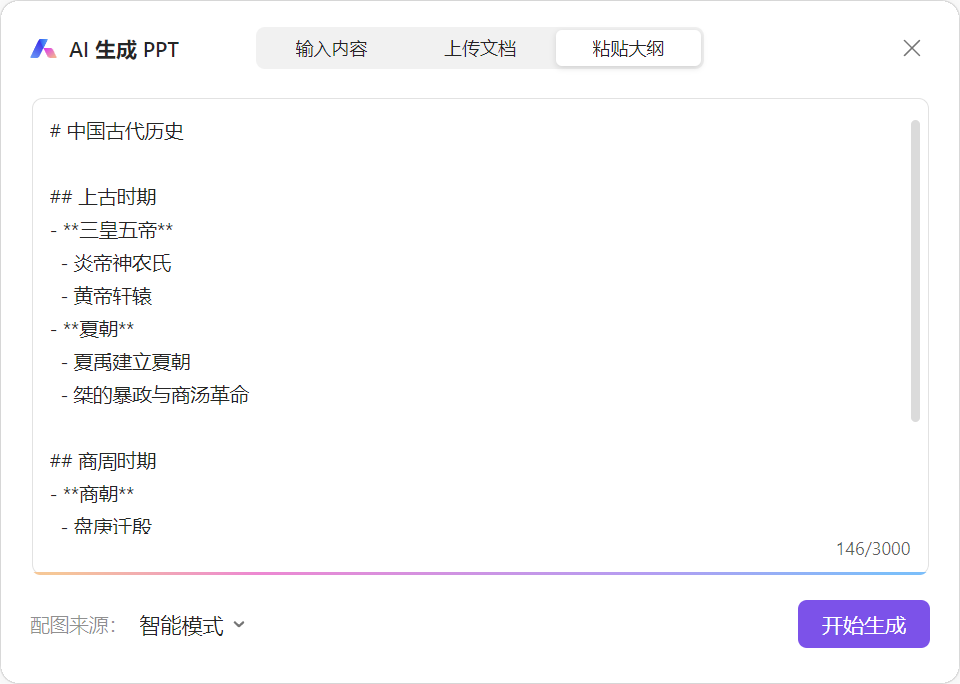
\includegraphics[width=0.7\textwidth]{sections/images/image-20250210192847219.png} %插入图片,[]中设置图片大小,{}中是图片文件名
    \caption{粘贴大纲到WPS} %最终文档中希望显示的图片标题
    \label{Fig.main1} %用于文内引用的标签
\end{figure}%结束环境

\centering
\begin{figure}[H] %H为当前位置,!htb为忽略美学标准,htbp为浮动图形
    \centering %图片居中
    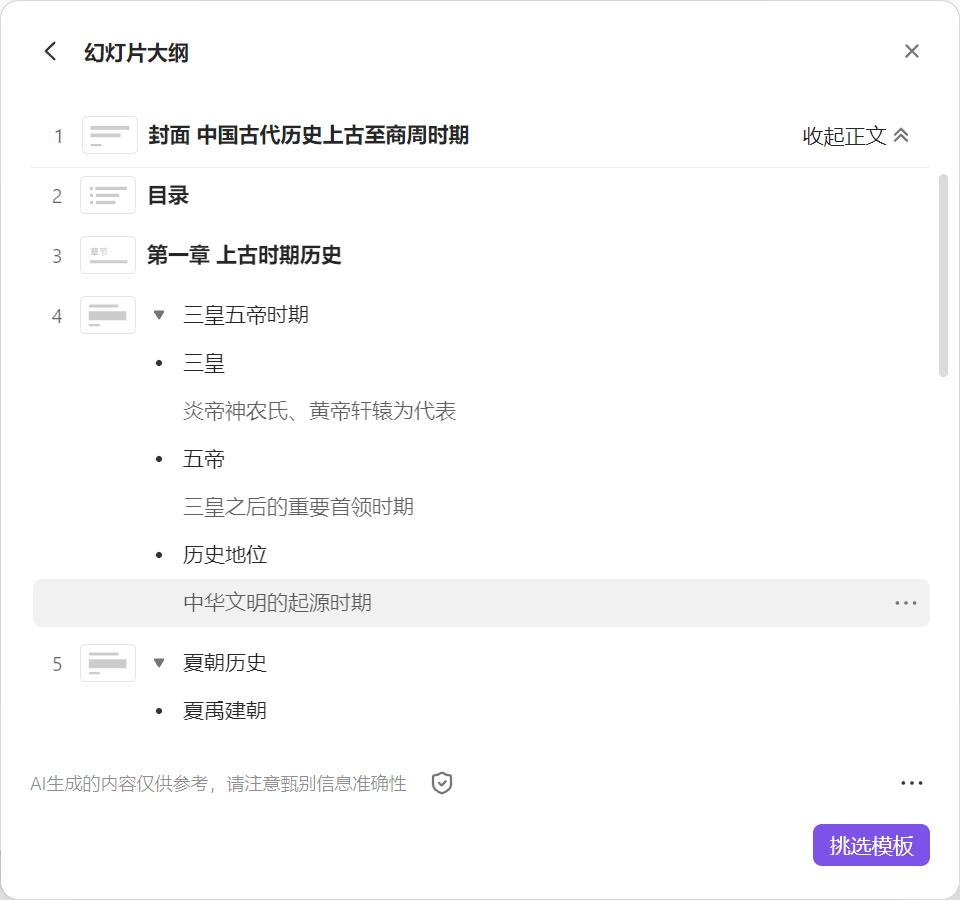
\includegraphics[width=0.7\textwidth]{sections/images/image-20250210192936323.png} %插入图片,[]中设置图片大小,{}中是图片文件名
    \caption{WPS生成大纲} %最终文档中希望显示的图片标题
    \label{Fig.main1} %用于文内引用的标签
\end{figure}%结束环境

\centering
\begin{figure}[H] %H为当前位置,!htb为忽略美学标准,htbp为浮动图形
    \centering %图片居中
    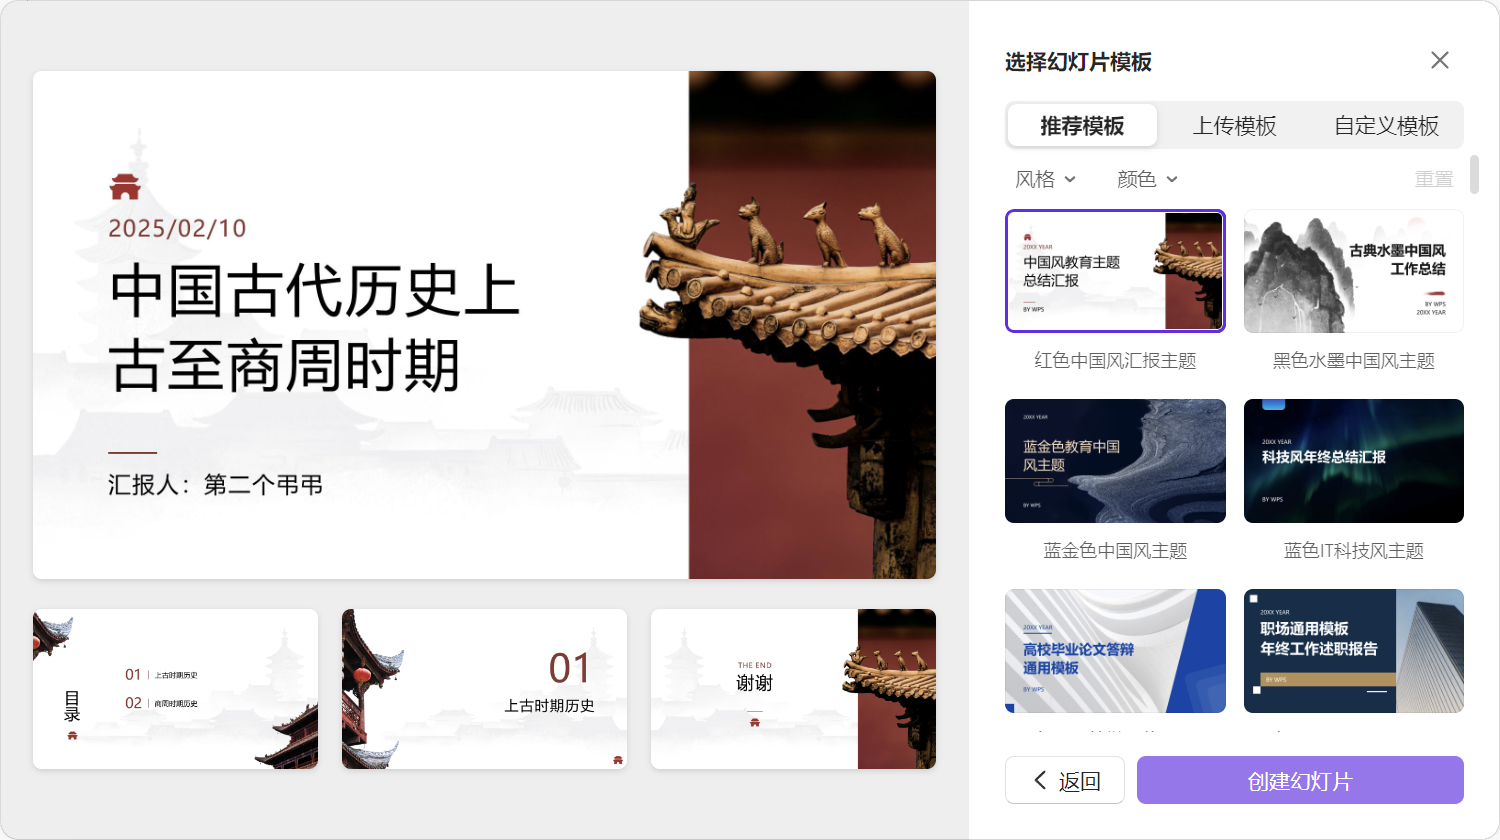
\includegraphics[width=0.7\textwidth]{sections/images/image-20250210192952252.png} %插入图片,[]中设置图片大小,{}中是图片文件名
    \caption{挑选合适的模板} %最终文档中希望显示的图片标题
    \label{Fig.main1} %用于文内引用的标签
\end{figure}%结束环境

\centering
\begin{figure}[H] %H为当前位置,!htb为忽略美学标准,htbp为浮动图形
    \centering %图片居中
    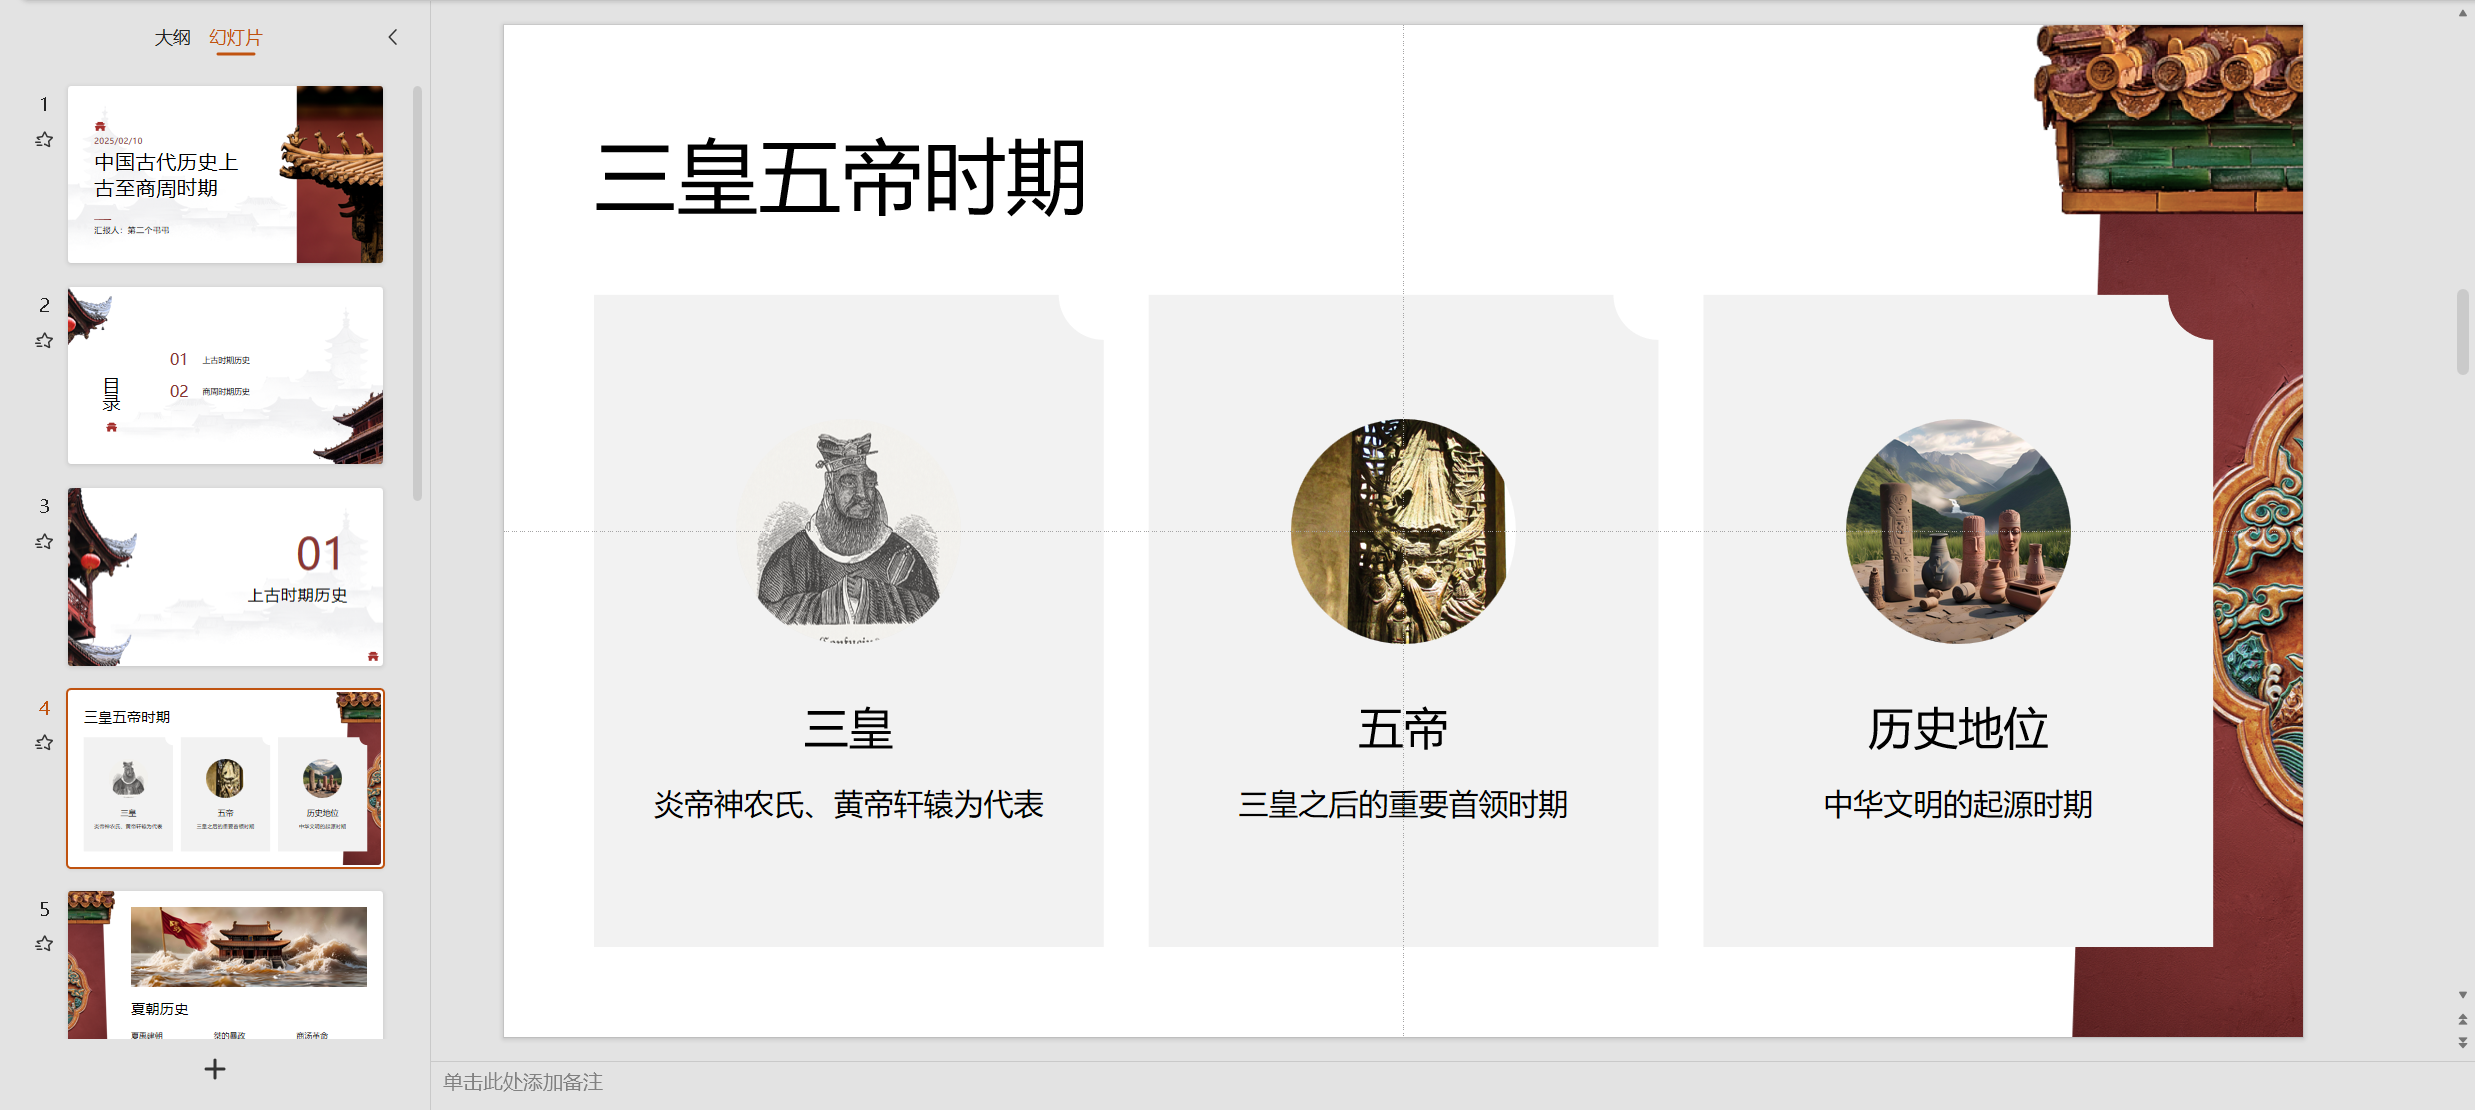
\includegraphics[width=0.7\textwidth]{sections/images/image-20250210193018631.png} %插入图片,[]中设置图片大小,{}中是图片文件名
    \caption{效果图} %最终文档中希望显示的图片标题
    \label{Fig.main1} %用于文内引用的标签
\end{figure}%结束环境

\textbf{步骤四:美化与调整}

\begin{itemize}

\item
  添加历史地图或重要人物画像。
\item
  使用时间轴展示各个朝代的更替。
\item
  在关键事件页面加入简短的动画效果,增强观众的理解和记忆。
\end{itemize}

\hypertarget{ux603bux7ed3}{%
\paragraph{总结}\label{ux603bux7ed3}}

通过GPT生成结构化的内容,并结合专业的PPT制作工具,我们可以高效地创建出内容丰富、设计美观的历史PPT。这种方法不仅节省时间,还能确保信息的准确性和呈现的专业性,特别适合文科生在学习和教学中使用。随着技术的发展,未来的工具将更加智能,帮助我们更轻松地完成复杂的任务。

\textbf{常见问题与建议}

\begin{itemize}

\item
  \textbf{准确性如何保证?}:在生成内容后,进行仔细校对,并参考权威的历史资料。
\item
  \textbf{复杂主题如何处理?}:可以分步查询GPT,逐步细化每个部分的内容,确保结构清晰。
\end{itemize}
